\documentclass{ximera}

\input{../../../preamble.tex}


\definecolor{fvdnavy}{HTML}{071D43}
\definecolor{fvdcyan}{HTML}{20BFC6}
\definecolor{fvdcyanlight}{HTML}{EFFCFB}
\definecolor{fvdmagenta}{HTML}{F10D69}
\definecolor{fvdmagentalight}{HTML}{FFF1F7}
\definecolor{fvdtext}{HTML}{163044}





%=================================================
% Pedagogische omgevingen
% PDF: tcolorbox
% HTML: learning-box
%=================================================

\newenvironment{voorkennis}
{%
    \ifdefined\HCode
        \HCode{%
<section class="learning-box learning-box--prior">
<div class="learning-box__header">
<span class="learning-box__icon" aria-hidden="true"></span>
<span class="learning-box__title">Voorkennis</span>
</div>
<div class="learning-box__content">
        }%
        \begin{itemize}
    \else
       \begin{tcolorbox}[
    enhanced,
    breakable,
    colback=fvdcyanlight,
    colframe=fvdcyan,
    coltext=fvdtext,
    boxrule=0.5pt,
    leftrule=4pt,
    arc=4mm,
    outer arc=4mm,
    left=7mm,
    right=6mm,
    top=5mm,
    bottom=5mm,
    before skip=6mm,
    after skip=6mm,
    title=Voorkennis,
    coltitle=fvdcyan,
    fonttitle=\bfseries\Large,
    attach title to upper={\par\smallskip},
    boxed title style={
        empty,
        left=0mm,
        right=0mm,
        top=0mm,
        bottom=0mm
    },
    overlay={
        \draw[
            fvdcyan,
            line width=0.5pt
        ]
        ([xshift=42mm,yshift=-13mm]frame.north west)
        --
        ([xshift=-7mm,yshift=-13mm]frame.north east);
    }
]
        \begin{itemize}
    \fi
}
{%
    \end{itemize}
    \ifdefined\HCode
        \HCode{%
</div>
</section>
        }%
    \else
        \end{tcolorbox}
    \fi
}


\newenvironment{leerdoelen}
{%
    \ifdefined\HCode
        \HCode{%
<section class="learning-box learning-box--goals">
<div class="learning-box__header">
<span class="learning-box__icon" aria-hidden="true"></span>
<span class="learning-box__title">Leerdoelen</span>
</div>
<div class="learning-box__content">
        }%
        \begin{itemize}
    \else
\begin{tcolorbox}[
    enhanced,
    breakable,
    colback=fvdmagentalight,
    colframe=fvdmagenta,
    coltext=fvdtext,
    boxrule=0.5pt,
    leftrule=4pt,
    arc=4mm,
    outer arc=4mm,
    left=7mm,
    right=6mm,
    top=5mm,
    bottom=5mm,
    before skip=6mm,
    after skip=6mm,
    title=Leerdoelen,
    coltitle=fvdmagenta,
    fonttitle=\bfseries\Large,
    attach title to upper={\par\smallskip},
    boxed title style={
        empty,
        left=0mm,
        right=0mm,
        top=0mm,
        bottom=0mm
    },
    overlay={
        \draw[
            fvdmagenta,
            line width=0.5pt
        ]
        ([xshift=42mm,yshift=-13mm]frame.north west)
        --
        ([xshift=-7mm,yshift=-13mm]frame.north east);
    }
]
        \begin{itemize}
    \fi
}
{%
    \end{itemize}
    \ifdefined\HCode
        \HCode{%
</div>
</section>
        }%
    \else
        \end{tcolorbox}
    \fi
}


\addPrintStyle{../../..}

\title{Oefeningen — Wanneer is een functie omkeerbaar?}
\author{Ingmar Herreman}

\begin{document}

% FVD_CHAPTER_DATA_START
% Automatisch gegenereerd uit index.tex.
% Niet handmatig aanpassen.
\fvdchapterdata{4}{Van relatie naar functie}{3}
% FVD_CHAPTER_DATA_END







\maketitle
\FVDbeginExercises


\begin{oefening}[Injectief, surjectief of bijectief?]{\oefB\ESS}

Onderzoek telkens de functie. Motiveer in termen van originelen en codomein.

\begin{question}
\[
f:\{1,2,3\}\to\{a,b,c\},
\qquad
f(1)=a,\ f(2)=b,\ f(3)=c.
\]

\begin{oplossing}
Iedere waarde in het codomein heeft precies één origineel.
De functie is injectief en surjectief, dus bijectief.
\end{oplossing}
\end{question}

\begin{question}
\[
g:\{1,2,3\}\to\{a,b\},
\qquad
g(1)=a,\ g(2)=b,\ g(3)=b.
\]

\begin{oplossing}
De functie is surjectief, want \(a\) en \(b\) worden bereikt.
Ze is niet injectief, want \(b\) heeft twee originelen.
Dus \(g\) is niet bijectief.
\end{oplossing}
\end{question}

\begin{question}
\[
h:\{1,2,3\}\to\{a,b,c,d\},
\qquad
h(1)=a,\ h(2)=b,\ h(3)=c.
\]

\begin{oplossing}
De functie is injectief, want geen uitvoer heeft twee originelen.
Ze is niet surjectief, want \(d\) wordt niet bereikt.
Dus \(h\) is niet bijectief.
\end{oplossing}
\end{question}

\end{oefening}

\begin{oefening}[Horizontale-lijntest]{\oefB\ESS}

Onderzoek grafisch of de functies injectief zijn.

\begin{question}
\[
f(x)=2x+1.
\]

\begin{oplossing}
Iedere horizontale lijn snijdt de grafiek hoogstens eenmaal.
De functie is injectief op \(\mathbb R\).
\end{oplossing}
\end{question}

\begin{question}
\[
g(x)=x^2.
\]

\begin{oplossing}
Niet injectief op \(\mathbb R\). Bijvoorbeeld \(y=4\) snijdt de grafiek
in \((-2,4)\) en \((2,4)\).
\end{oplossing}
\end{question}

\begin{question}
\[
h(x)=|x|.
\]

\begin{oplossing}
Niet injectief op \(\mathbb R\). Voor iedere \(b>0\) heeft \(b\)
twee originelen, \(b\) en \(-b\).
\end{oplossing}
\end{question}

\end{oefening}

\begin{oefening}[Bereik en codomein]{\oefB\ESS}

Beschouw
\[
f(x)=x^2.
\]

\begin{question}
Is
\[
f:\mathbb R\to\mathbb R
\]
surjectief?

\begin{oplossing}
Nee. Het bereik is \([0,+\infty[\), terwijl het codomein \(\mathbb R\) is.
Negatieve reële getallen worden niet bereikt.
\end{oplossing}
\end{question}

\begin{question}
Is
\[
g:\mathbb R\to[0,+\infty[:x\mapsto x^2
\]
surjectief?

\begin{oplossing}
Ja. Het bereik is gelijk aan het codomein \([0,+\infty[\).
\end{oplossing}
\end{question}

\begin{question}
Zijn \(f\) en \(g\) injectief?

\begin{oplossing}
Nee. In beide gevallen is het domein \(\mathbb R\) en geldt bijvoorbeeld
\[
(-2)^2=2^2.
\]
\end{oplossing}
\end{question}

\end{oefening}

\begin{oefening}[Bijectief maken]{\oefB\ESS}

Beschouw
\[
f(x)=x^2.
\]

\begin{question}
Waarom is \(f:\mathbb R\to[0,+\infty[\) niet bijectief?

\begin{oplossing}
De functie is wel surjectief maar niet injectief.
Positieve functiewaarden hebben twee originelen.
\end{oplossing}
\end{question}

\begin{question}
Vul domein en codomein aan zodat hetzelfde voorschrift een bijectie wordt:
\[
g:\ldots\to\ldots:x\mapsto x^2.
\]

\begin{oplossing}
Bijvoorbeeld
\[
g:[0,+\infty[\to[0,+\infty[:x\mapsto x^2.
\]
Ook
\[
g:]-\infty,0]\to[0,+\infty[
\]
is mogelijk.
\end{oplossing}
\end{question}

\begin{question}
Verklaar je keuze grafisch.

\begin{oplossing}
Op elk gekozen halfdomein snijdt iedere horizontale lijn \(y=b\) met \(b\geq0\)
de grafiek precies eenmaal. Iedere waarde van het codomein heeft dus precies
één origineel.
\end{oplossing}
\end{question}

\end{oefening}



\begin{oefening}[Dezelfde formule, andere functie]{\oefU\ESS}

Beschouw telkens het voorschrift \(x\mapsto x^2\).

\[
f:\mathbb R\to\mathbb R,
\]
\[
g:\mathbb R\to[0,+\infty[,
\]
\[
h:[0,+\infty[\to\mathbb R,
\]
\[
k:[0,+\infty[\to[0,+\infty[.
\]

Maak een tabel waarin je voor elke functie aangeeft of ze injectief,
surjectief en bijectief is. Motiveer.

\begin{oplossing}
\[
\begin{array}{c|ccc}
&\text{injectief}&\text{surjectief}&\text{bijectief}\\
\hline
f&\text{nee}&\text{nee}&\text{nee}\\
g&\text{nee}&\text{ja}&\text{nee}\\
h&\text{ja}&\text{nee}&\text{nee}\\
k&\text{ja}&\text{ja}&\text{ja}
\end{array}
\]

Dit toont dat bijectiviteit niet alleen van het voorschrift afhangt,
maar van de volledige functie met domein en codomein.
\end{oplossing}

\end{oefening}

\begin{oefening}[GeoGebra: zoek zelf een domeinbeperking]{\oefU\ESS}

Teken in GeoGebra
\[
f(x)=(x-2)^2-1.
\]

Maak een schuifknop \(b\) en teken \(y=b\).

\begin{question}
Waarom is \(f\) op \(\mathbb R\) niet injectief?

\begin{oplossing}
Horizontale lijnen boven \(y=-1\) snijden de parabool tweemaal.
De overeenkomstige functiewaarden hebben dus twee originelen.
\end{oplossing}
\end{question}

\begin{question}
Geef twee verschillende maximale intervallen waarop de functie wel injectief is.

\begin{oplossing}
\[
]-\infty,2]
\qquad\text{en}\qquad
[2,+\infty[.
\]
\end{oplossing}
\end{question}

\begin{question}
Welk codomein kies je bij beide beperkingen om een bijectie te verkrijgen?

\begin{oplossing}
Het bereik op beide intervallen is
\[
[-1,+\infty[.
\]
Dat kiezen we als codomein.
\end{oplossing}
\end{question}

\end{oefening}

\begin{oefening}[Grafiek zonder voorschrift]{\oefU\ESS}

Beschouw de grafiek.

\begin{center}
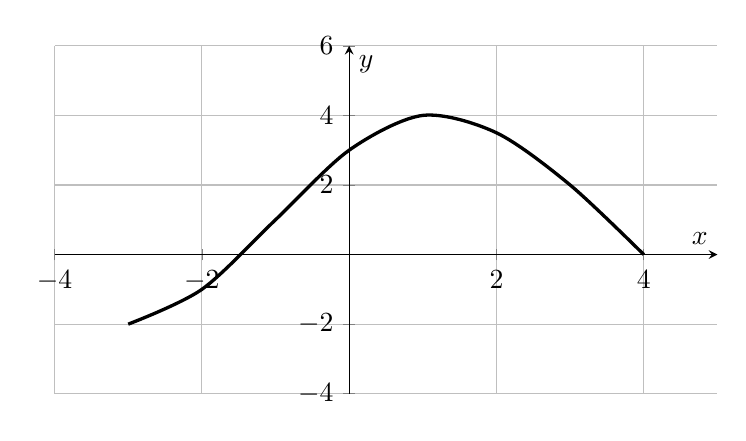
\begin{tikzpicture}
\begin{axis}[
width=10cm,height=6cm,
xmin=-4,xmax=5,ymin=-4,ymax=6,
xlabel={$x$},ylabel={$y$},
axis lines=middle,grid=both]
\addplot[very thick,smooth] coordinates {(-3,-2)(-2,-1)(-1,1)(0,3)(1,4)(2,3.5)(3,2)(4,0)};
\end{axis}
\end{tikzpicture}
\end{center}

\begin{question}
Is de functie injectief op het getekende domein? Motiveer uitsluitend vanuit de grafiek.

\begin{oplossing}
Nee. Er bestaan horizontale lijnen die de grafiek tweemaal snijden,
bijvoorbeeld een lijn met een \(y\)-waarde tussen ongeveer \(0\) en \(4\).
\end{oplossing}
\end{question}

\begin{question}
Geef een mogelijk deelinterval waarop de functie wel injectief is.

\begin{oplossing}
Bijvoorbeeld het gedeelte van \(x=-3\) tot \(x=1\), of het gedeelte van
\(x=1\) tot \(x=4\), afgelezen uit de grafiek.
\end{oplossing}
\end{question}

\end{oefening}

\begin{oefening}[Sensor: kan je de invoer reconstrueren?]{\oefU\ESS}

Een sensor zet een grootheid \(x\) om in een signaal
\[
S(x)=x^2,
\qquad -5\leq x\leq5.
\]

\begin{question}
Kan je uit de uitlezing \(S=16\) de oorspronkelijke \(x\)-waarde eenduidig bepalen?

\begin{oplossing}
Nee:
\[
x=-4\quad\text{of}\quad x=4.
\]
De sensorcodering is op dit domein niet injectief.
\end{oplossing}
\end{question}

\begin{question}
Welke informatie gaat verloren?

\begin{oplossing}
Het teken van de oorspronkelijke waarde. Positieve en negatieve waarden
met dezelfde absolute waarde leveren hetzelfde signaal.
\end{oplossing}
\end{question}

\begin{question}
Geef een domeinbeperking waardoor reconstructie wel eenduidig wordt.

\begin{oplossing}
Bijvoorbeeld
\[
0\leq x\leq5
\]
of
\[
-5\leq x\leq0.
\]
\end{oplossing}
\end{question}

\end{oefening}



\begin{oefening}[Ontwerp een bijectie]{\oefG}

Gegeven zijn
\[
A=\{1,2,3,4\},
\qquad
B=\{a,b,c,d\}.
\]

\begin{question}
Hoeveel pijlen moet een bijectie \(f:A\to B\) bevatten?
Welke voorwaarden moeten de pijlen vervullen?

\begin{oplossing}
Er zijn vier pijlen. Uit ieder element van \(A\) vertrekt precies één pijl
en in ieder element van \(B\) komt precies één pijl aan.
\end{oplossing}
\end{question}

\begin{question}
Teken twee verschillende bijecties \(A\to B\).

\begin{oplossing}
Er zijn veel mogelijkheden, bijvoorbeeld
\[
1\mapsto a,\ 2\mapsto b,\ 3\mapsto c,\ 4\mapsto d
\]
en
\[
1\mapsto d,\ 2\mapsto a,\ 3\mapsto c,\ 4\mapsto b.
\]
\end{oplossing}
\end{question}

\end{oefening}

\begin{oefening}[Omkeerbaarheid zonder formule]{\oefG}

Een meettoestel zet een fysische grootheid \(q\) om in een elektrische
uitgangsspanning \(U\). Uit een kalibratiegrafiek blijkt dat \(U\) eerst
toeneemt met \(q\), een maximum bereikt en daarna opnieuw afneemt.

Zonder een concreet functievoorschrift te kennen:

\begin{enumerate}
    \item leg uit waarom de volledige kalibratiefunctie vermoedelijk niet injectief is;
    \item beschrijf grafisch hoe je dat controleert;
    \item leg uit hoe je een bruikbaar meetbereik zou kunnen kiezen waarin
          de invoer uit de uitgangsspanning wel eenduidig kan worden gereconstrueerd;
    \item formuleer welke extra voorwaarde aan het codomein nodig is om van
          een bijectie te spreken.
\end{enumerate}

\begin{oplossing}
Voor spanningen onder het maximum kunnen doorgaans twee waarden van \(q\)
dezelfde spanning opleveren. Een horizontale lijn snijdt de kalibratiegrafiek
dan tweemaal. Men kan één monotone tak van de grafiek als werkgebied kiezen,
zodat iedere toegelaten spanning hoogstens één origineel heeft. Om bijectief
te zijn moet het gekozen codomein bovendien precies samenvallen met het bereik
op dat werkgebied.
\end{oplossing}

\end{oefening}



\end{document}
